% !TeX spellcheck = en_US

% We need layers to draw the block diagram
\usetikzlibrary{calc,positioning}

% Define a few styles and constants
\tikzstyle{entry}=[draw, fill=green!20, minimum height=2.0em, minimum width=8.0em]
\tikzstyle{ann} = [above, text width=5em]
\tikzstyle{framework} = [entry, text width=35em, fill=red!20, 
minimum height=18em, rounded corners]
\tikzstyle{lang} = [entry, text width=9em, fill=blue!20, 
minimum height=15em, rounded corners]
\def\blockdist{2.3}
\def\edgedist{2.5}

\begin{figure}
	\centering
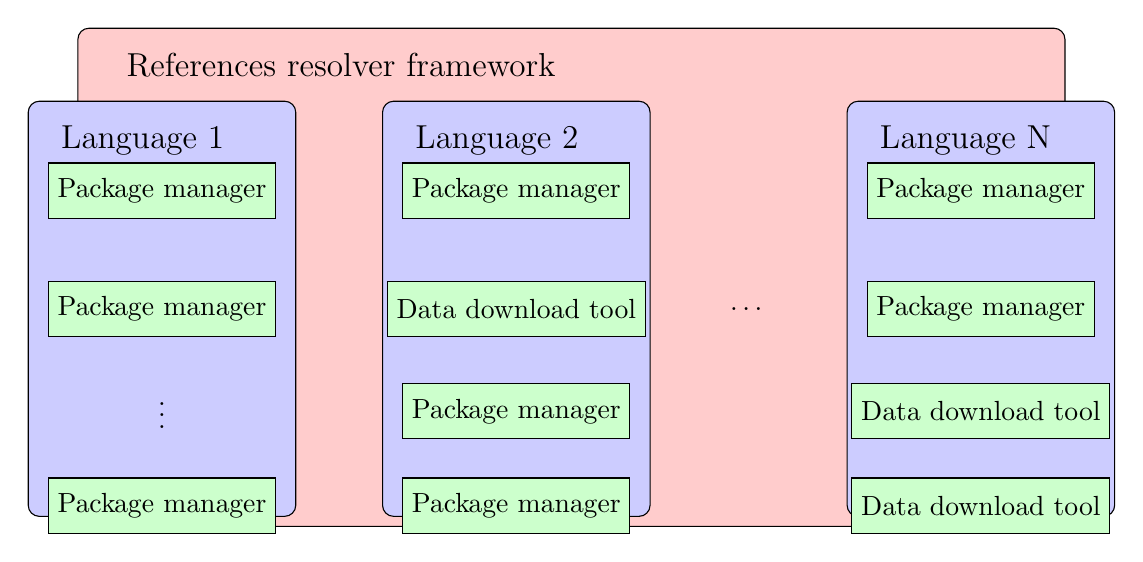
\begin{tikzpicture}
\node (rr) [framework] {};
\node [xshift=+5mm, yshift=-2mm, below right] at (rr.north west) {\large References resolver framework };


\node (lang1) at ([xshift=-52mm,yshift=-4mm]rr) [lang] {};
\node [xshift=+3mm, yshift=-2mm, below right] at (lang1.north west) {\large Language 1 };
\node (lang2) at ([xshift=-7mm,yshift=-4mm]rr) [lang] {};
\node [xshift=+3mm, yshift=-2mm, below right] at (lang2.north west) {\large Language 2 };
\node (langn) at ([xshift=+52mm,yshift=-4mm]rr) [lang] {};
\node [xshift=+3mm, yshift=-2mm, below right] at (langn.north west) {\large Language N };
\node at ($(lang2)!.5!(langn)$) {\ldots};

\node (l1pm1) at ([yshift=+15mm]lang1) [entry] {Package manager};
\node (l1pm2) at ([yshift=0mm]lang1) [entry] {Package manager};
\node (l1pmn) at ([yshift=-25mm]lang1) [entry] {Package manager};
\node at ($(l1pm2)!.5!(l1pmn)$) {\vdots};

\node (l2pm1) at ([yshift=+15mm]lang2) [entry] {Package manager};
\node (l2pm2) at ([yshift=0mm]lang2) [entry] {Data download tool};
\node (l2pm3) at ([yshift=-13mm]lang2) [entry] {Package manager};
\node (l2pmn) at ([yshift=-25mm]lang2) [entry] {Package manager};
%\node at ($(l2pm2)!.5!(l2pmn)$) {\vdots};

\node (lnpm1) at ([yshift=+15mm]langn) [entry] {Package manager};
\node (lnpm2) at ([yshift=0mm]langn) [entry] {Package manager};
\node (lnpm3) at ([yshift=-13mm]langn) [entry] {Data download tool};
\node (lnpmn) at ([yshift=-25mm]langn) [entry] {Data download tool};
%\node at ($(lnpm2)!.5!(lnpmn)$) {\vdots};


\end{tikzpicture} 
\caption{An example scheme representing several language modules containing package manager modules} 	\label{fig:lang_pm}
\end{figure}